\chapter{Modellierung und Evaluation}

Die Modellierung in dieser Phase erfolgt \emph{zunächst} auf Basis der in Phase~04 (alter Ansatz) ermittelten, EPV-konformen Merkmalsmengen je Horizont. Die verschachtelten Ergebnisse (H1 bereits vorliegend) werden nach Abschluss als Sensitivitäts- und Robustheitsvergleich ergänzt (``alte Auswahl'' vs. ``nested-basierte Auswahl'').

\section{Modellarchitekturen}

\subsection{Baseline: Logistische Regression}
Eingesetzt wird eine Pipeline aus \texttt{StandardScaler} und logistischer Regression mit L2-Regularisierung (Solver \texttt{lbfgs}). Die Parameter folgen Phase~05: \mbox{$C=1{,}0$}, \texttt{class\_weight=balanced}, \texttt{max\_iter=100000}, \texttt{tol=$10^{-3}$}, \texttt{random\_state=42}. Die Konfiguration ist über alle Horizonte identisch, um Vergleichbarkeit zu wahren. Die Bewertung erfolgt mit 5-fach stratifizierter Cross-Validation; Primärmetrik ist ROC-AUC, PR-AUC dient als Imbalance-sensitive Zweitmetrik.

\subsection{Random Forest}
Als baumbasierte Referenz wird ein \texttt{RandomForestClassifier} genutzt. Parameter (aus der Projektkonfiguration): \texttt{n\_estimators=800}, \texttt{max\_depth=20}, \texttt{min\_samples\_split=10}, \texttt{min\_samples\_leaf=5}, \texttt{max\_features="sqrt"}, \texttt{class\_weight="balanced\_subsample"}, \texttt{n\_jobs=6}, \texttt{random\_state=42}. Diese Einstellungen sind für alle Horizonte konstant. Der Ansatz ist robust gegenüber Multi\-kollinearität und liefert verlässliche Wahrscheinlichkeits-Scores für AUC-basierte Bewertung.

\subsection{Gradient Boosting und weitere Modelle}
Zusätzlich werden in Phase~05b weitere Verfahren geprüft: \texttt{GradientBoostingClassifier} (\texttt{random\_state=42}), \texttt{ExtraTreesClassifier} (Parameter analog RF inkl. \texttt{class\_weight}), sowie \texttt{SVC} in einer Skalierungs-Pipeline (\texttt{probability=True}, \texttt{class\_weight=balanced}, \texttt{random\_state=42}). Ein Soft-Voting-Ensemble kombiniert LR(L2, skaliert) + GB + ET (\texttt{voting="soft"}). Es findet keine umfangreiche Hyperparameter-Suche statt; die Konfiguration ist bewusst moderat und reproduzierbar gehalten.


\section{Hyperparameter-Tuning}
In Phase~05 erfolgt \emph{keine} breit angelegte Hyperparameter-Optimierung. Ziel ist eine faire, replizierbare Gegenüberstellung der Modellfamilien unter EPV- und Rechenzeit-Gesichtspunkten. RF nutzt feste, in der Konfiguration dokumentierte Einstellungen; LR verwendet die o.\,g. Standardparameter. Für die Extra-Modelle werden ebenso konservative Defaults eingesetzt. Ausführliches Tuning und Kalibrierung sind als Erweiterung vorgesehen (vgl. Kap.~\ref{chap:future-work}).

\subsection{Cross-Validation}
Alle Modelle werden je Horizont mit 5-fach \emph{stratifizierter} CV evaluiert (\texttt{shuffle=True}, \texttt{random\_state=42}). Bewertet wird anhand vorhergesagter \emph{Wahrscheinlichkeiten} (nicht Klassenlabels); Primärmetrik ist ROC-AUC, ergänzt um PR-AUC. Nested-CV wird in Phase~04 für die Feature-Selektion genutzt; die Modellvergleiche in Phase~05 erfolgen mit einheitlicher, nicht-verschachtelter CV zur transparenten Gegenüberstellung der Verfahren.

\subsection{Horizontspezifisches Tuning}
Spezifische Tuning-Schritte pro Horizont wurden \emph{nicht} durchgeführt. Die Parameter bleiben konstant; Unterschiede in der Güte entstehen aus daten- und prävalenzbedingten Horizontunterschieden. Dies gewährleistet Vergleichbarkeit der Modelle über H1–H5.


\section{Behandlung der Klassenimbalance}
Die Klassenungleichgewichte werden über \texttt{class\_weight} adressiert: LR nutzt \texttt{balanced}, RF \texttt{balanced\_subsample}, SVC \texttt{balanced}. Es kommen \emph{keine} Resampling-Verfahren zum Einsatz. Schwellen werden nicht optimiert; stattdessen werden schwellenunabhängige Flächenmetriken (ROC-/PR-AUC) berichtet. Kalibrierung und geschäftsfallbezogene Schwellenwahl folgen in Kap.~\ref{chap:future-work}.

\section{Ergebnisse}
% Automatisch generierte Zusammenfassungstabelle der besten Modelle je Horizont
% Auto-generated by generate_phase05_tables.py
\begin{table}[H]
  \centering
  \caption{Modellgüte pro Horizont (beste ROC-AUC und PR-AUC)}
  \label{tab:phase05_modeling_summary}
  \begin{tabular}{l l r r r}
    \toprule
    Horizont & Bestes Modell & ROC-AUC & PR-AUC & Anzahl Features \\
    \midrule
    H1 & softvote\_lr\_gb\_et & 0.796 & 0.183 & 10 \\
    H2 & random\_forest & 0.845 & 0.341 & 9 \\
    H3 & random\_forest & 0.780 & 0.140 & 7 \\
    H4 & random\_forest & 0.812 & 0.218 & 8 \\
    H5 & random\_forest & 0.864 & 0.420 & 10 \\
    \bottomrule
  \end{tabular}
\end{table}
\medskip

Zusätzlich fasst Tabelle~\ref{tab:phase05_modeling_comparison} die jeweils besten Baseline-Modelle (LR/RF) den besten Extra-/Ensemble-Varianten sowie dem insgesamt besten Verfahren je Horizont gegenüber (primäre Optimierung: ROC-AUC). Dadurch wird transparent, in welchen Horizonten Ensemble- oder Boosting-Modelle die Baselines übertreffen und wo die lineare Referenz konkurrenzfähig bleibt.

\input{tables/phase05_modeling_comparison}

\subsection*{Ergänzende Gesamtübersicht}
\input{tables/phase06_model_eval_matrix_wrapped}

Kurzfazit (ROC-AUC, insgesamt Bestes je Horizont): H1 gewinnt das Soft-Voting-Ensemble (0{,}796), H2--H5 jeweils der Random Forest (0{,}845/0{,}780/0{,}812/0{,}864); damit dominiert der Random Forest in vier von fünf Horizonten, das Ensemble liegt in H1 knapp vorn.

\paragraph{PR-AUC der Sieger-Modelle.}
Ergänzend zur ROC-AUC werden die im Klassenungleichgewicht aussagekräftigeren PR-AUC-Werte berichtet \parencite{saito2015precision}. Für die jeweils bestplatzierten Modelle je Horizont ergeben sich: H1~(Soft-Voting)~0{,}183; H2~(Random Forest)~0{,}341; H3~(Random Forest)~0{,}140; H4~(Random Forest)~0{,}218; H5~(Random Forest)~0{,}420 (vgl. Tab.~\ref{tab:phase05_modeling_summary}). Die Werte sind konsistent mit der beobachteten Zunahme der Zielklassenprävalenz über die Horizonte (vgl. Kap.~3): PR-AUC steigt in späteren Horizonten tendenziell an.

\begin{figure}[H]
\centering
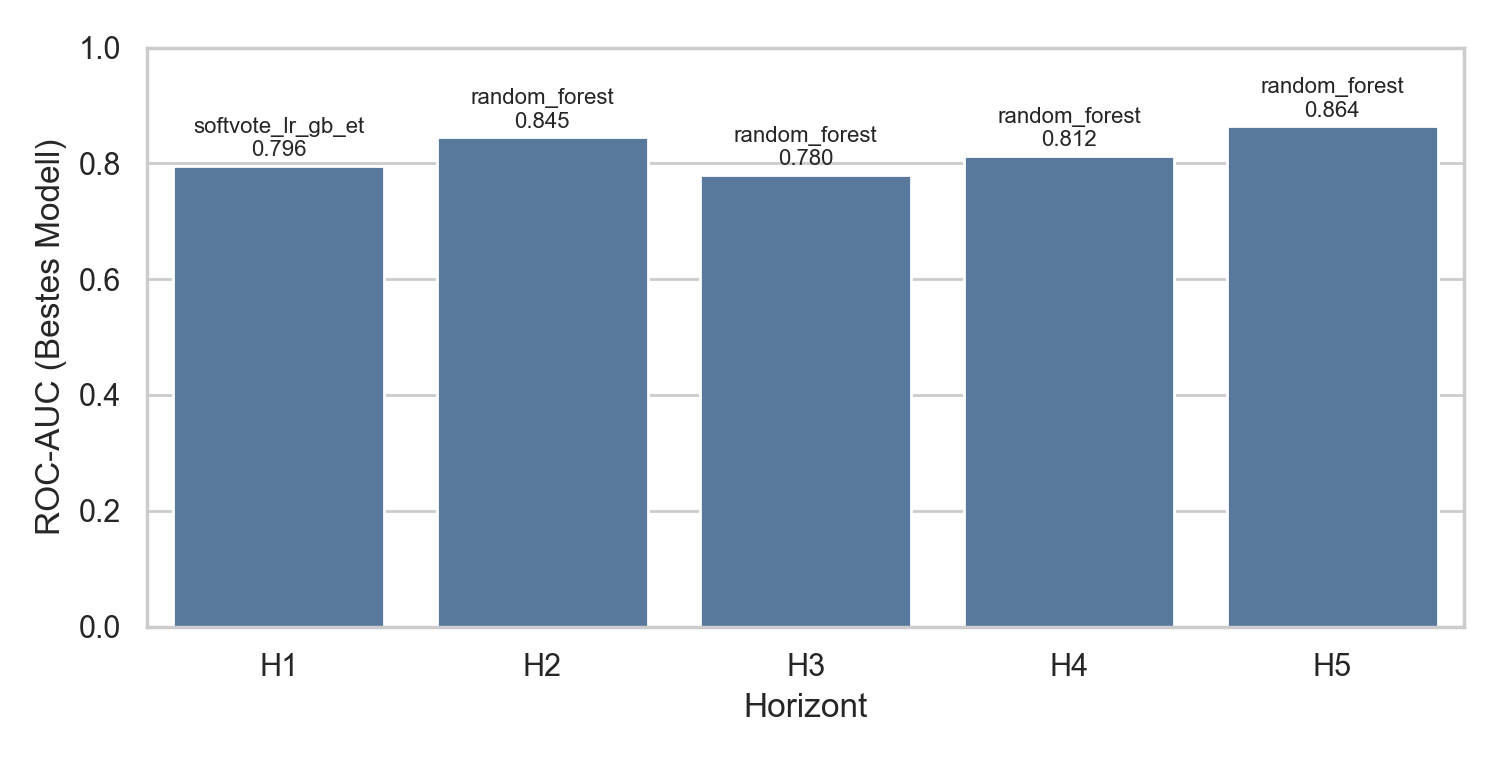
\includegraphics[width=0.88\textwidth]{figures/phase05/model_best_auc.png}
\caption{Bestes Modell und ROC-AUC je Horizont}
\label{fig:phase05_best_auc}
\par\smallskip
{\footnotesize Quelle: Eigene Darstellung basierend auf \texttt{results/05\_modeling/} und \texttt{extra/}}
\end{figure}


\paragraph{Hinweis zur Kalibrierung und Schwellenwahl.}
In dieser Phase wurden bewusst \emph{keine} Wahrscheinlichkeitskalibrierung (Platt/Isoton) und \emph{keine} geschäftsfallbezogene Schwellenoptimierung vorgenommen. Beides ist als eigenständiger Schritt mit klarer Kostenfunktion zu behandeln und wird in Kap.~\ref{chap:future-work} als zukünftige Erweiterung vorgesehen. Für die vergleichende Bewertung werden daher primär schwellenunabhängige Flächenmetriken (ROC-/PR-AUC) herangezogen.

\subsection*{Abweichung zu archivierten Performanzangaben}
Im historischen Archiv wird für den polnischen Datensatz ein Wert von ``0{,}9812 (98{,}12\% accuracy)'' ausgewiesen (CatBoost, Einzel-Split). Diese Zahl ist aus heutigen Kriterien als \emph{explorativ und potenziell optimistisch} zu klassifizieren. Die wichtigsten Ursachen der Abweichung gegenüber den hier berichteten, moderateren ROC-AUC-Werten (ca. 0{,}80--0{,}86) sind:
\begin{itemize}
	\item \textbf{Validierungsregime:} Archiv: einzelner Train/Test-Split ohne Wiederholungs- oder Faltungseffekte; hier: 5-fach stratifizierte Cross-Validation reduziert Varianz und Optimismus.
	\item \textbf{Metrik-Bezeichnung:} Im Archiv wird ROC-AUC mit ``Accuracy'' semantisch vermischt, was einen höheren Anschein klassifikatorischer Exaktheit suggeriert als tatsächlich vorliegt.
	\item \textbf{Feature-Selektion / EPV:} Archiv nutzte vor EPV-Remediation breitere, teils multikollineare Merkmalslisten; hier strikt EPV-konforme, redundanzreduzierte Sets (geringerer Overfit-Spielraum).
	\item \textbf{Modellkomplexität:} CatBoost (gradient boosting mit kategorialer Spezialbehandlung) war archiviert inkludiert und vermutlich feinjustiert; in dieser Phase wurde aus Reproduzierbarkeits- und Ressourcen-Gründen auf ein begrenztes, transparentes Set (LR, RF, GB, SVC, ExtraTrees, Voting) fokussiert.
	\item \textbf{Potenzielle Leckagen:} Einzel-Split ohne temporale Sensitivitätsprüfung erhöht Risiko strukturierter Zufallsartefakte; aktuelle Pipeline vermeidet dies durch methodische Reihenfolge (Foundation -> Selektion -> CV).
	\item \textbf{Klassenimbalance-Behandlung:} Archivwerte können von ungeeigneten Schwellen oder unkalibrierten Wahrscheinlichkeiten profitieren; hier werden class\_weight-Adjustments konsistent angewandt und primär Schwellen-unabhängige Flächenmetriken (ROC-/PR-AUC) berichtet.
\end{itemize}
In Summe stellen die hier dokumentierten Ergebnisse eine \emph{konservativere, robustere und publizierbare} Schätzung der generalisierbaren Modellgüte dar. Die archivierte CatBoost-Performanz ist als explorativer Obergrenz-Hinweis zu interpretieren, nicht als belastbare Replikationsbasis.
